\documentclass[aspectratio=1610]{beamer}
\usepackage{theme}
\usepackage[utf8x]{inputenc}

\usepackage[english]{babel}
\usepackage{calligra}
\usepackage{lmodern}
\usepackage{subcaption}
\usepackage{hyperref}

\usepackage{amsmath,amssymb,amsfonts,physics}
\usepackage{array, booktabs, makecell}
\usepackage{tabularx}

\usepackage{textcomp}
\makeatletter
\newcommand{\removelatexerror}{\let\@latex@error\@gobble}
\makeatother

% Graphics and video
\usepackage{graphicx,float,wrapfig}
\graphicspath{
  {./assets/images/}%
}


% args: big, bigg, Big, Bigg
\newcommand{\parenth}[2][]{#1(#2#1)}
\renewcommand{\bold}[1]{\textbf{\structure{#1}}}
  
\author[Daniotti \and Lucerno]{Filippo Daniotti \and Taylor Lucerno}
\title[NeRF-W]{\textsc{NeRF in the Wild}}
\subtitle{Neural Radiance Fields for Unconstrained Photo Collections}
\institute[DISI - UniTN]{Department of Information Engineering\\and Computer Science}
\date{\today}


\AtBeginSection[]
{
    \begin{frame}
        \frametitle{Table of Contents}
        \tableofcontents[currentsection]
    \end{frame}
}

\begin{document}

\begin{frame}
    \titlepage
    \begin{figure}[H]
        \begin{center}
            
\includegraphics[width=0.4\linewidth]{marchio_unitrento_colore_it_202002.eps}
        \end{center}
    \end{figure}
\end{frame}


\begin{frame}
    \tableofcontents[sectionstyle=show,subsectionstyle=show/shaded/hide,subsubsectionstyle=show/shaded/hide]
\end{frame}

\section{Introduction}
\begin{frame}{Introduction}
    Content:
    \begin{itemize}
        \item problem statement
        \item NeRF
        \item NeRF in the Wild
    \end{itemize}
\end{frame}

\section{The Problem}
\begin{frame}
    \begin{itemize}
        \item synthesizing novel views of a scene from a sparse set of captured images
        \item doing it in unconstrained environment:
        \begin{itemize}
            \item scene varies amongst training set (illumination, shading, tone)
            \item scene is partially occluded by obstacles
        \end{itemize}
    \end{itemize}
\end{frame}

\section{Background: Neural Radiance Fields}
\begin{frame}{Core concepts: representing a scene as a NeRF}
    \begin{block}{In a nutshell}
        NeRFs represent a continuous complex scene as a function 
        \begin{equation*}
            F_\theta : (\vb{x}, \vb{d}) \rightarrow (\vb{c}, \sigma)
        \end{equation*}
    \end{block}
    This function is approximated with a MLP \(F_\theta \rightarrow\)  overfitted to encode only scene!
    % \pause
    \bigskip
    \begin{figure}[H]
        \centering
        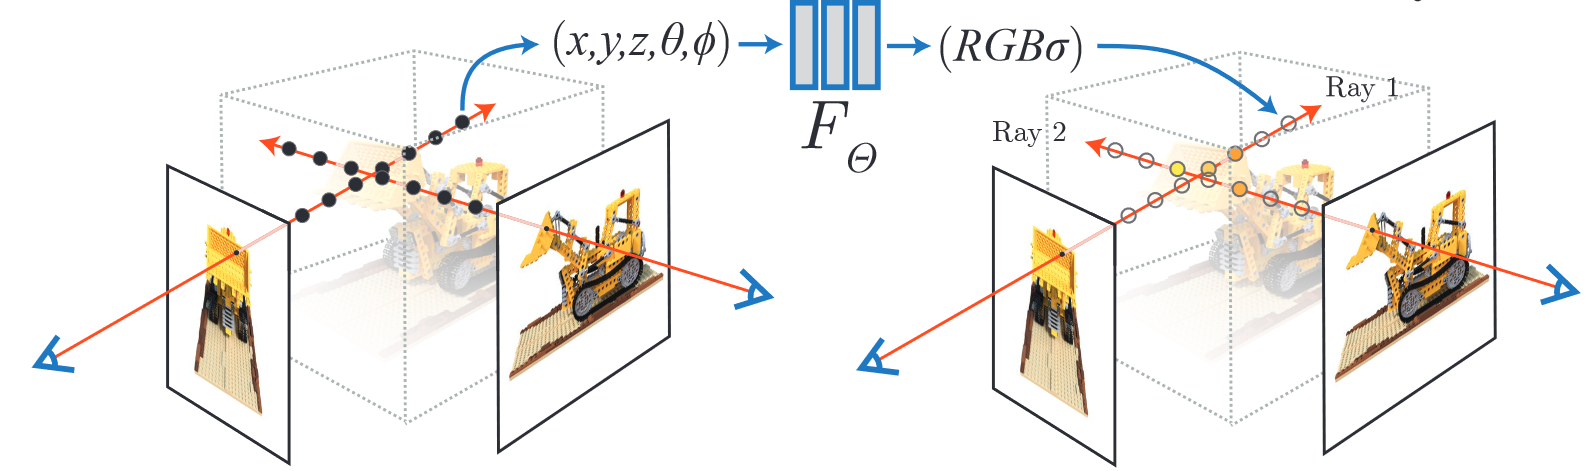
\includegraphics[width=.7\textwidth,keepaspectratio]{mapping}
    \end{figure}
\end{frame}

\begin{frame}{Core concepts: synthesizing novel views}
    \begin{columns}
        \begin{column}{.5\textwidth}
            \begin{figure}[H]
                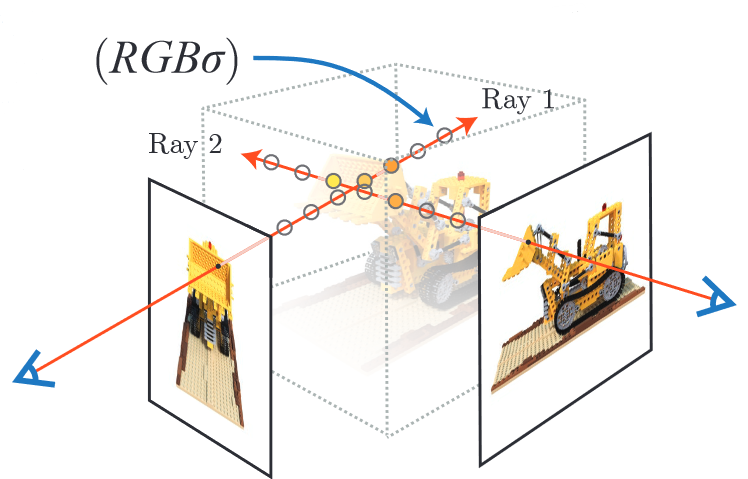
\includegraphics[width=.7\textwidth,keepaspectratio]{density-1}
            \end{figure}
        \end{column}
        \pause
        \begin{column}{.5\textwidth}
            \begin{figure}[H]
                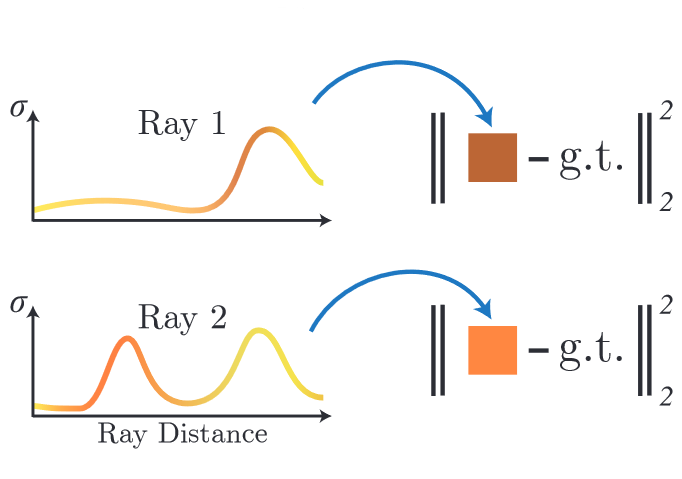
\includegraphics[width=.7\textwidth,keepaspectratio]{density-2}
            \end{figure}
        \end{column}
    \end{columns}
    \begin{onlyenv}<3->
        \begin{block}{Volume rendering with Radiance Fields} 
            Approximate the expected color \(\hat{\vb{C}}(\vb{r})\) encountered by camera ray \(\vb{r}(t) = \vb{o} + t\vb{d}\)
            \begin{equation*}
                \hat{\vb{C}}(\vb{r}) = \mathcal{R}(\vb{r}, \vb{c}, \sigma) = \sum_{k = 1}^{K} T(t_k) \alpha (\sigma (t_k)\delta_k) \vb{c}(t_k)
            \end{equation*}
        \end{block}
    \end{onlyenv}
\end{frame}

\begin{frame}{Architecture}
    \begin{onlyenv}<1>
        \begin{figure}[H]
            \centering
            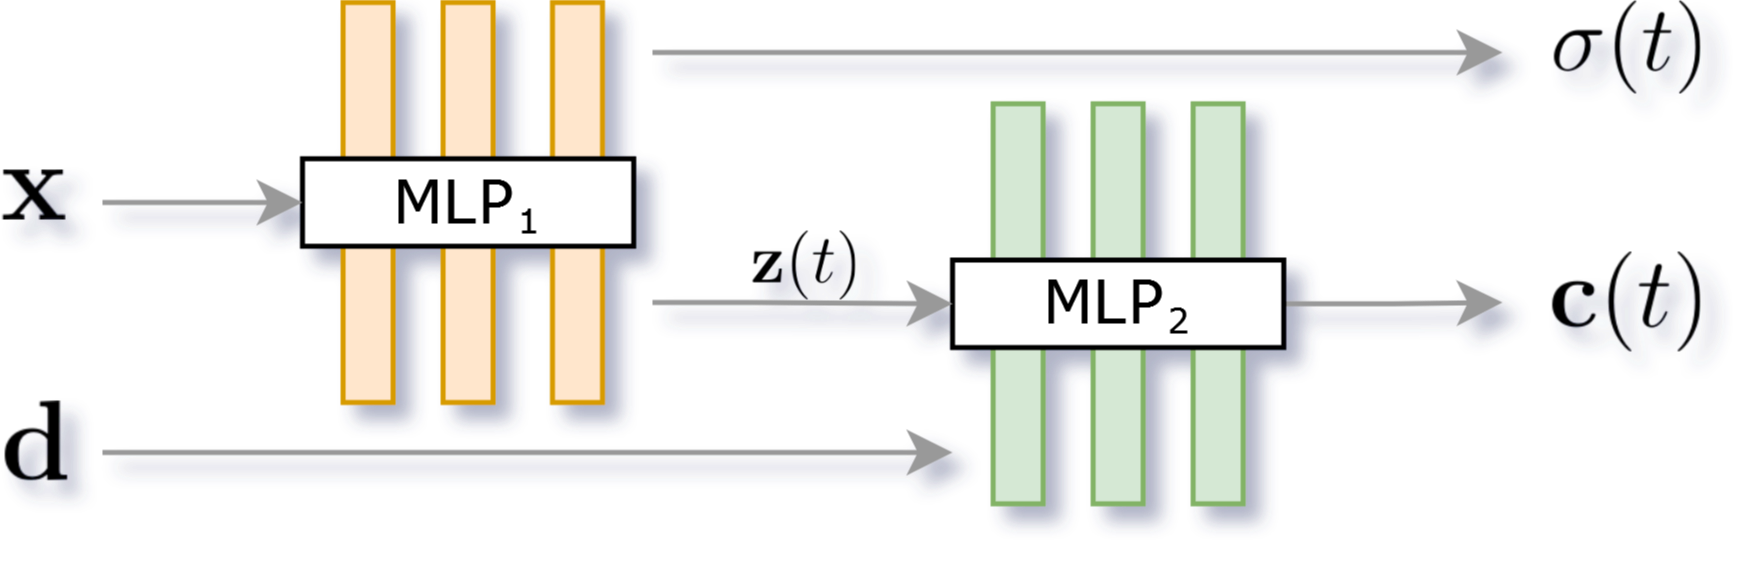
\includegraphics[width=.8\textwidth]{nerf-architecture}
        \end{figure}
    \end{onlyenv}

    \pause
    
    \begin{onlyenv}<2->
        \begin{columns}
            \begin{column}{.7\textwidth}
                \begin{figure}[H]
                    \centering
                    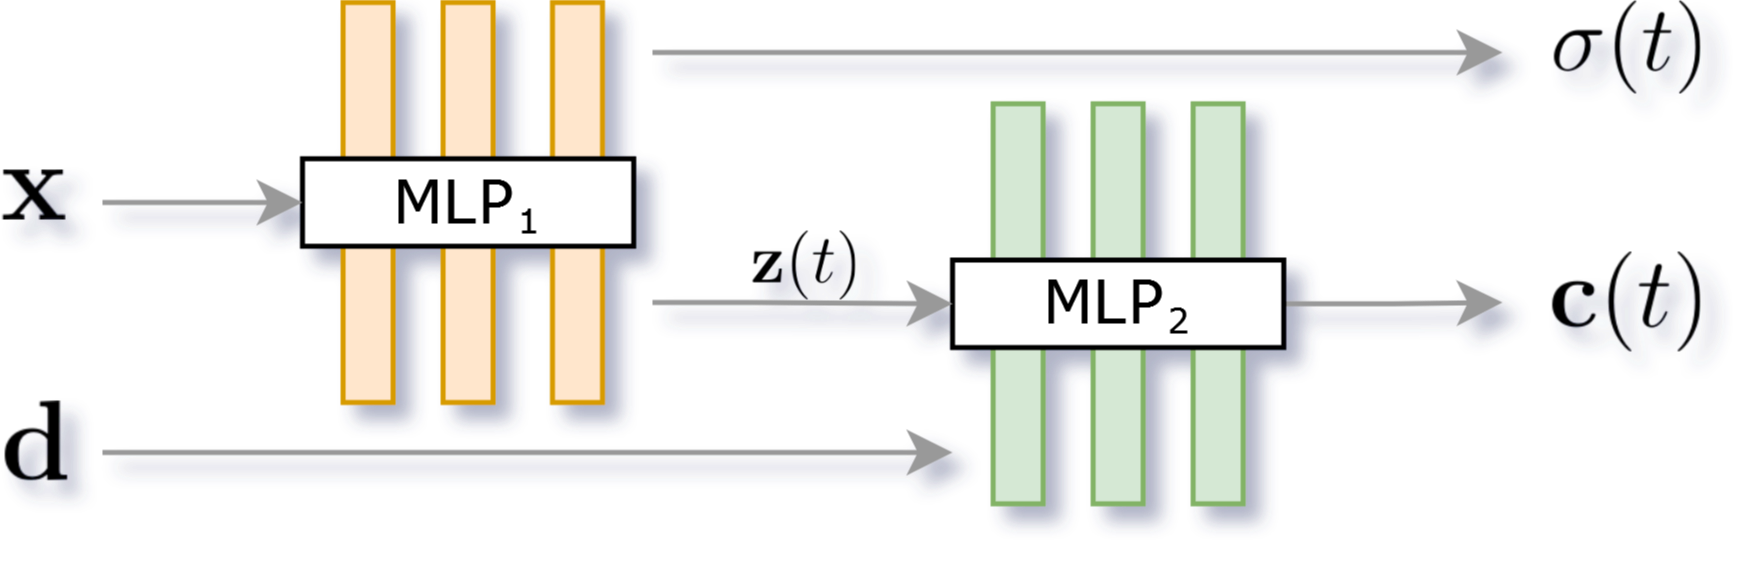
\includegraphics[width=.65\textwidth]{nerf-architecture}
                \end{figure}
            \end{column}
            \begin{column}{.3\textwidth}
                \Large{Why?}
            \end{column}
        \end{columns}
        \vspace{1.2cm}

        \pause

        \uncover<3->{
            \begin{columns}
                \begin{column}{.3\textwidth}
                    \centering
                    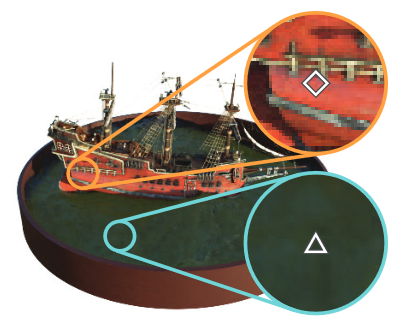
\includegraphics[width=.75\textwidth]{architecture-why-1.png}
                \end{column}
                \pause
                \begin{column}{.3\textwidth}
                    \centering
                    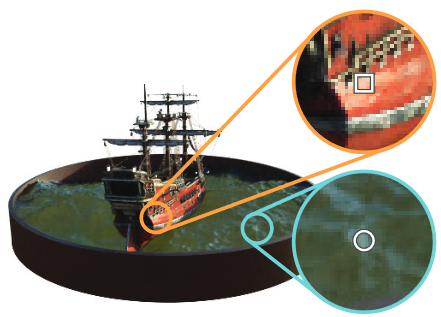
\includegraphics[width=.75\textwidth]{architecture-why-2.png}
                \end{column}
                \pause
                \begin{column}{.3\textwidth}
                    \centering
                    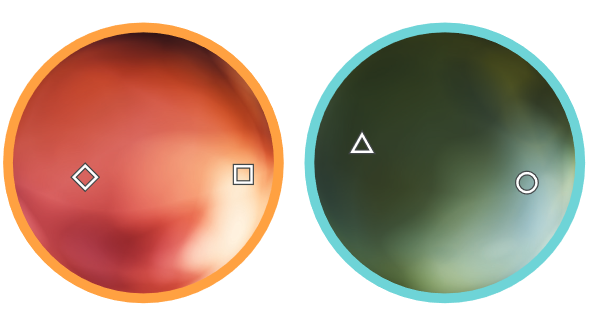
\includegraphics[width=.9\textwidth]{architecture-why-3.png}
                \end{column}
            \end{columns}
        }
    \end{onlyenv}
    % Quick note on the architecture:
    % \begin{itemize}
    %     \item the original NeRF uses one single MLP
    %     \item NeRF-W uses two different MLPs the better enforce the dependencies
    %     \begin{itemize}
    %         \item one to estimate density \(\sigma(t)\) and a vector \(\vb{z}(t)\) from the location
    %         \item one to estimate the color \(\vb{c}(t)\) from the viewing direction and the vector \(\vb{z}(t)\)
    %     \end{itemize}
    % \end{itemize}
    % \begin{block}{MLPs}
    %     \begin{align}
    %         [\sigma(t), \vb{z}(t)] &= \textrm{MLP}_{\theta_1} (\gamma_{\vb{x}}(\vb{r}(t))) \\
    %         \vb{c}(t) &= \textrm{MLP}_{\theta_2} (\vb{z}(t), \gamma_{\vb{d}}(\vb{d}))
    %     \end{align}
    % \end{block}
\end{frame}

\begin{frame}{Optimizing NeRFs}
    A few tricks are employed
    \bigskip
    \pause
    \begin{columns}[t]
        \begin{column}{.4\textwidth}
            \textbf{Positional encoding}\\
            map \(\vb{x}\) and \(\vb{d}\) to a higher-dimensional space
            \begin{align*}
                &\textrm{MLP}_{\theta_1} (\gamma_{\vb{x}}(\vb{x})) \\
                &\textrm{MLP}_{\theta_2} (\vb{z}(t), \gamma_{\vb{d}}(\vb{d}))
            \end{align*}
        \end{column}
        \pause
        \begin{column}{.4\textwidth}
            \textbf{Hierarchical volume sampling}\\
            use 2 MLPs sequentially
            \begin{align*}
                &\vb{\hat{C}}^c(\vb{r}) \rightarrow \textrm{coarse one}\\
                &\vb{\hat{C}}^f(\vb{r}) \rightarrow \textrm{fine one}
            \end{align*}
        \end{column}
    \end{columns}
    % \begin{itemize}
    %     \item Positional encoding: location vector \(\vb{x}\) is mapped to a higher dimensional space in order to more easily approximate higher-frequency functions
    %     \item Hierarchical volume sampling: two MLP are actually employed, a coarse one (first) and then a fine one (sampling points for its rays are sampled after the coarse has run for a given training epoch) 
    % \end{itemize}
    \bigskip
    \pause
    \begin{block}{Training objective}
        \begin{equation}
            \sum_{\vb{r} \in \mathcal{R}} ||\vb{C}(\vb{r}) - \vb{\hat{C}}^c(\vb{r})||_2^2 + ||\vb{C}(\vb{r}) - \vb{\hat{C}}^f(\vb{r})||_2^2
        \end{equation}
    \end{block}
\end{frame}

\begin{frame}{NeRF Limitations}
    NeRFs assume real world scenes to be \textbf{static}
    \vspace{1.5cm}
    \begin{columns}[t]
        \begin{column}{.4\textwidth}
            Phonometric variations\\
        \end{column}
        \begin{column}{.4\textwidth}
            Transient objects\\
        \end{column}
    \end{columns}
    \begin{columns}
        \begin{column}{.4\textwidth}
            \begin{center}
                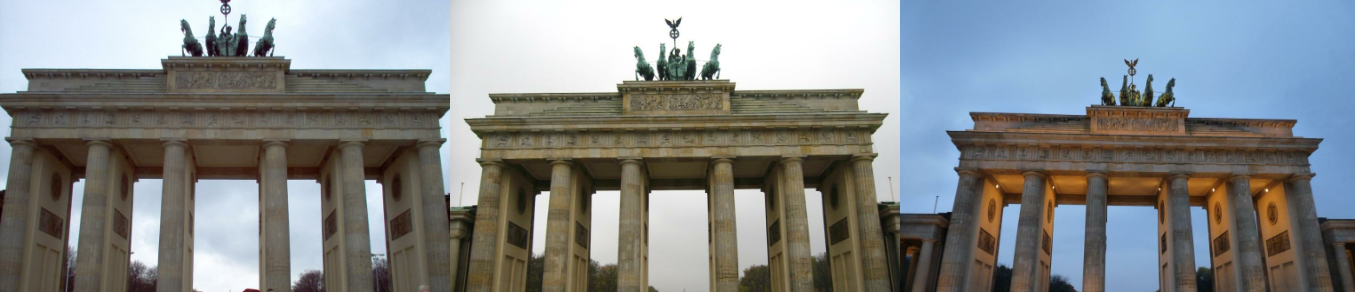
\includegraphics[width=\textwidth]{issues-var.png}
            \end{center}
        \end{column}
        \begin{column}{.4\textwidth}
            \begin{center}
                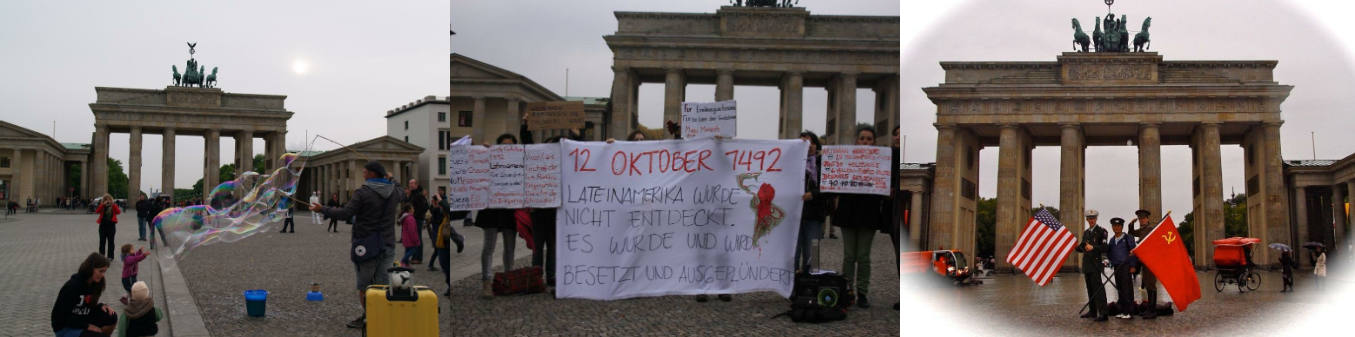
\includegraphics[width=\textwidth]{issues-transient.png}
            \end{center}
        \end{column}
    \end{columns}
    % \begin{itemize}
    %     \item phonometric variations: two photographs of a scene taken at different times of day, different periods of the year, atmospheric conditions will vary in terms of illumination, shading, ton quality
    %     \item transient objects: many real world landmakrs will have a crowd around, possibly captured in the shots
    % \end{itemize}
    \vspace{1.5cm}
    \pause
    NeRF in the wild addresses these two issues
\end{frame}

\section{Paper contribution: NeRF in the Wild}
\begin{frame}{}

    

\end{frame}

\section{Limitations, possible improvements, future work}
\begin{frame}[plain,noframenumbering]
    \begin{center}
        Thanks for your attention
    \end{center}
\end{frame}

\end{document}